

\section*{Introduction to absolute values}

This year, you will be introduced to many kinds of functions.
One of them is \emph{absolute value}.
This is a confusing function, because of its notation.

\begin{center}
    \begin{tcolorbox}[width=3.5in]
        The {\bfseries\itshape absolute value} of $x$ is written with $x$ 
        between {\bfseries\itshape vertical bars} like this:
        \[   |x|   \]
    \end{tcolorbox}
\end{center}

There are two ways to explain the absolute value: algebraic and geometric.

\begin{center}
    \begin{tcolorbox}[width=5in]
    The {\bfseries\itshape algebraic definition} of $|x|$ is:
    \[ 
        |x| \equiv
        \begin{cases} 
            x &  \text{if } x>0 \qquad\text{\itshape this will be a positive number, since $x$ is positive}\\
            0 &  \text{if } x=0 \\
            -x & \text{if } x<0 \qquad\text{\itshape this will be a positive number also}
        \end{cases}
    \]
    
    The result is {\bfseries\itshape always} positive (or zero).
    \end{tcolorbox}
    \end{center}

    \begin{center}
        \begin{tcolorbox}[width=5in]
            The {\bfseries\itshape geometric definition} of $|x|$ uses \emph{distance} on a numberline.
            \vskip1em
            The absolute value of a number tells you how far it is from the origin (either to the left or to the right).
            This is a \emph{distance} which is {\bfseries\itshape always positive}.\footnote{
                How far are you from Bastrop if you are 10 miles east? 10 miles.
                How far are you from Bastrop if you are 10 miles west? 10 miles.
                In both case, the answer is \emph{positive 10}.
            }
            \vskip1em
            The following number line illustrates this for $x=2$ and $x=-2$. Both points are $2$ units away from the origin.
            This is what $|x|=2$ means --- that whatever $x$ is, 
            it is two units away from the origin 
            (maybe to the left, maybe to the right)
            \vspace{1em}
            
            \begin{center}
                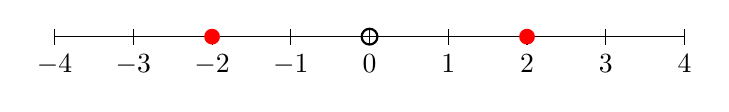
\begin{tikzpicture}
                    \draw (-4,0) -- (4,0);
                    \foreach \i in {-4,-3,...,4} % numbers on line
                    \draw (\i,0.1) -- + (0,-0.2) node[below] {$\i$}; % tick and their labels
                    \foreach \i in {0}% points on line
                    \draw[black,thick] (\i,0) circle (0.1 cm);
                    \foreach \i in {-2,2}% points on line
                    \fill[red] (\i,0) circle (0.1 cm);
                \end{tikzpicture}
            \end{center}
        \end{tcolorbox}
        \end{center}
            


